\documentclass{article} % A4 paper and 11pt font size
\setcounter{secnumdepth}{0}

\usepackage{amssymb, amsmath, amsfonts}
\usepackage{moreverb}
\usepackage{multicol}
\usepackage{graphicx}
\usepackage{enumerate}
\usepackage{changepage}
\usepackage{lipsum}
\usepackage{caption}
\usepackage{nicefrac}
\usepackage{graphics}
\usepackage[margin=1in]{geometry}
\usepackage{tocloft}
\renewcommand{\cftsecleader}{\cftdotfill{\cftdotsep}}
\usepackage{array}
\usepackage{arydshln}
\usepackage{float}
\usepackage{subcaption}
\usepackage{csquotes}
\usepackage{placeins}
\usepackage{verbatim}
\usepackage{hyperref}
\usepackage{textcomp}
\usepackage[makeroom]{cancel}
\usepackage{bbold}
\usepackage{scrextend}
\usepackage{alltt}
\usepackage[utf8]{inputenc}
\usepackage{listings}
\usepackage{color}
\usepackage{physics}
\usepackage{mathtools}
\usepackage[normalem]{ulem}
\usepackage{amsthm}
\usepackage{tikz}
\usetikzlibrary{positioning}
\usetikzlibrary{arrows}
\usepackage{pgfplots}
\usepackage{bigints}
\allowdisplaybreaks
\pgfplotsset{compat=1.12}

\theoremstyle{plain}
\newtheorem*{theorem*}{Theorem}
\newtheorem{theorem}{Theorem}
\newtheorem*{lemma*}{Lemma}
\newtheorem{lemma}{Lemma}

\definecolor{verbgray}{gray}{0.9}
% \definecolor{dkgreen}{green}{0.9}

\lstdefinestyle{PythonCode}{%
  language=Python,
  backgroundcolor=\color{verbgray},
  keywordstyle=\color{blue},      % keyword style
  keywordstyle=[2]\color{blue},   % keyword style
  commentstyle=\color{magenta},   % comment style
  stringstyle=\color{olive},      % string literal styleframe=single,
  numberstyle=\color{black},      % string literal styleframe=single,
  framerule=0pt,
  numbers=left,
  stepnumber=1,
  firstnumber=1,
  showspaces=false,
  basicstyle=\ttfamily}

\lstset{style=PythonCode}

\makeatletter
\newcommand{\BIGG}{\bBigg@{3}}
\newcommand{\vast}{\bBigg@{4}}
\newcommand{\Vast}{\bBigg@{5}}
\makeatother

\newenvironment{definition}[1][Definition]{\begin{trivlist}
\item[\hskip \labelsep {\bfseries #1}]}{\end{trivlist}}

\newcommand{\dy}{\partial_y}
\newcommand{\dyy}{\partial_{yy}}
\newcommand{\dxx}{\partial_{xx}}
\newcommand{\dxy}{\partial_{xy}}
\newcommand{\dyyy}{\partial_{yyy}}
\newcommand{\dxxx}{\partial_{xxx}}
\newcommand{\dx}{\partial_x}
\newcommand{\E}{\varepsilon}
\def\Rl{\mathbb{R}}
\def\Cx{\mathbb{C}}

\newcommand{\Ei}{\text{Ei}}

\usepackage[T1]{fontenc} % Use 8-bit encoding that has 256 glyphs
\usepackage{fourier} % Use the Adobe Utopia font for the document - comment this line to return to the LaTeX default
\usepackage[english]{babel} % English language/hyphenation

\usepackage{sectsty} % Allows customizing section commands
\allsectionsfont{\centering \normalfont\scshape} % Make all sections centered, the default font and small caps

\usepackage{fancyhdr} % Custom headers and footers
\pagestyle{fancy} % Makes all pages in the document conform to the custom headers and footers
\fancyhead[L]{\bf Sam Fleischer}
\fancyhead[C]{\bf UC Davis \\ Numerical Solutions of Differential Equations (MAT228B)} % No page header - if you want one, create it in the same way as the footers below
\fancyhead[R]{\bf Winter 2017}

\fancyfoot[L]{\bf } % Empty left footer
\fancyfoot[C]{\bf \thepage} % Empty center footer
\fancyfoot[R]{\bf } % Page numbering for right footer
\renewcommand{\headrulewidth}{0pt} % Remove header underlines
\renewcommand{\footrulewidth}{0pt} % Remove footer underlines
\setlength{\headheight}{25pt} % Customize the height of the header

\newcommand{\VEC}[2]{\left\langle #1, #2 \right\rangle}
\newcommand{\ran}{\text{\rm ran }}
\newcommand{\Hilb}{\mathcal{H}}
\newcommand{\lap}{\Delta}

\newcommand{\Dx}{\Delta x}
\newcommand{\Dt}{\Delta t}

\newcommand{\littleo}[1]{\text{\scriptsize$\mathcal{O}$}\qty(#1)}

\DeclareMathOperator*{\esssup}{\text{ess~sup}}

\newcommand{\problem}[2]{
\vspace{.375cm}
\boxed{\begin{minipage}{\textwidth}
    \section{\bf #1}
    #2
\end{minipage}}
}

\numberwithin{equation}{section} % Number equations within sections (i.e. 1.1, 1.2, 2.1, 2.2 instead of 1, 2, 3, 4)
\numberwithin{figure}{section} % Number figures within sections (i.e. 1.1, 1.2, 2.1, 2.2 instead of 1, 2, 3, 4)
\numberwithin{table}{section} % Number tables within sections (i.e. 1.1, 1.2, 2.1, 2.2 instead of 1, 2, 3, 4)

\setlength\parindent{0pt} % Removes all indentation from paragraphs - comment this line for an assignment with lots of text

\newcommand{\horrule}[1]{\rule{\linewidth}{#1}} % Create horizontal rule command with 1 argument of height

\title{ 
\normalfont \normalsize 
\textsc{UC Davis, Numerical Solutions of Differential Equations (MAT 228B), Winter 2017} \\ [25pt] % Your university, school and/or department name(s)
\horrule{2pt} \\[01.4cm] % Thin top horizontal rule
\Huge Homework \#3 \\ % The assignment title
\horrule{2pt} \\[0.5cm] % Thick bottom horizontal rule
}

\author{\huge Sam Fleischer} % Your name

\date{March 3, 2017} % Today's date or a custom date

\begin{document}\thispagestyle{empty}

\maketitle % Print the title

\makeatletter
\@starttoc{toc}
\makeatother

\pagebreak

\problem{Problem 1}{Consider
\begin{gather*}
    u_t = 0.1\laplacian u \text{ on } \Omega = (0,1)\times(0,1) \\
    \frac{\partial u}{\partial \vec{n}} = 0 \text{ on } \partial\Omega \\
    u(x,y,0) = \exp(-10\qty(\qty(x - 0.3)^2 + \qty(y - 0.4)^2)).
\end{gather*}
Write a program to solve this PDE using the Peaceman-Rachford ADI scheme on a cell-centered grid.  Use a direct solver for the tridiagonal systems.  In a cell-centered discretization the solution is stored at the grid points $(x_i,y_i) = \qty(\Dx\qty(i - 0.5),\Dx\qty(j - 0.5))$ for $i,j = 1,\dots,N$ and $\dx = \frac{1}{N}$.  This discretization is natural for handling Neumann boundary conditions, and it is often used to discretize conservation laws.  At the grid points adjacent to the boundary, the one-dimensional discrete Laplacian for homogeneous Neumann boundary conditions is $$u_{xx}(x_1) \approx \frac{-u_1 + u_2}{\Dx^2}.$$
\begin{enumerate}[\ \ (a)]
    \item Perform a refinement study to show that your numerical solution is second-order accurate in space and time (refine time and space simultaneously using $\Dt = \Dx$) at time $t = 1$.
    \item Time your code for different grid sizes.  Show how the computational time scales with the grid size.  Compare your timing results with those from the previous homework assignment for Crank-Nicolson.
    \item Show that the spatial integral of the solution to the PDE does not change in time.  That is, $$\frac{\dd}{\dd t}\int_\Omega u \dd V = 0.$$
    \item Show that the solution to the discrete equations satisfies the discrete conservation property $$\sum_{i,j}u_{i,j}^n = \sum_{i,j}u_{i,j}^0$$ for all $n$.  Demonstrate this property with your code.
\end{enumerate}}

\begin{enumerate}[\ \ (a)]
    \item
        When we use methods which don't utilize cell-centered grids, it is easiest to do a refinement study using a grid spacing of $2^n$ since every other point in the finer mesh is in the same location as a point from the coarser mesh.  In cell-centered grids, however, halving $\Dx$ moves where we are sampling our functions, so it is easiest to do a refinement study using a grid spacing of $3^n$ since every third point in the finer mesh is in the same location as a point from the coarser mesh.  This is displayed below where large black points are the locations of coarse sampling and small red circles are the locations of fine sampling.
        \begin{figure}[ht!]
            \centering
            \begin{tikzpicture}
                \draw[step=1cm,gray,line width=0.05mm] (0,0) grid (4,4);
                \draw[step=2cm,gray,line width=0.75mm] (0,0) grid (4,4);
                \foreach \Point in {
                    (1,1),(1,3),(3,3),(3,1)}
                    \draw[fill=black] \Point circle (0.15);
                \foreach \Point in {
                    (0.5,0.5),(0.5,1.5),(0.5,2.5),(0.5,3.5),
                    (1.5,0.5),(1.5,1.5),(1.5,2.5),(1.5,3.5),
                    (2.5,0.5),(2.5,1.5),(2.5,2.5),(2.5,3.5),
                    (3.5,0.5),(3.5,1.5),(3.5,2.5),(3.5,3.5)
                    }
                    \draw[fill=red,line width=0mm] \Point circle (0.05);
            \end{tikzpicture}$\qquad\qquad$ vs.\hfill
            \begin{tikzpicture}
                \draw[step=1cm,gray,line width=0.05mm] (0,0) grid (9,9);
                \draw[step=3cm,gray,line width=0.75mm] (0,0) grid (9,9);
                \foreach \Point in {
                    (1.5,1.5),(1.5,4.5),(1.5,7.5),
                    (4.5,1.5),(4.5,4.5),(4.5,7.5),
                    (7.5,1.5),(7.5,4.5),(7.5,7.5)}
                    \draw[fill=black] \Point circle (0.15);
                \foreach \Point in {
                    (0.5,0.5),(0.5,1.5),(0.5,2.5),(0.5,3.5),(0.5,4.5),(0.5,5.5),(0.5,6.5),(0.5,7.5),(0.5,8.5),
                    (1.5,0.5),(1.5,1.5),(1.5,2.5),(1.5,3.5),(1.5,4.5),(1.5,5.5),(1.5,6.5),(1.5,7.5),(1.5,8.5),
                    (2.5,0.5),(2.5,1.5),(2.5,2.5),(2.5,3.5),(2.5,4.5),(2.5,5.5),(2.5,6.5),(2.5,7.5),(2.5,8.5),
                    (3.5,0.5),(3.5,1.5),(3.5,2.5),(3.5,3.5),(3.5,4.5),(3.5,5.5),(3.5,6.5),(3.5,7.5),(3.5,8.5),
                    (4.5,0.5),(4.5,1.5),(4.5,2.5),(4.5,3.5),(4.5,4.5),(4.5,5.5),(4.5,6.5),(4.5,7.5),(4.5,8.5),
                    (5.5,0.5),(5.5,1.5),(5.5,2.5),(5.5,3.5),(5.5,4.5),(5.5,5.5),(5.5,6.5),(5.5,7.5),(5.5,8.5),
                    (6.5,0.5),(6.5,1.5),(6.5,2.5),(6.5,3.5),(6.5,4.5),(6.5,5.5),(6.5,6.5),(6.5,7.5),(6.5,8.5),
                    (7.5,0.5),(7.5,1.5),(7.5,2.5),(7.5,3.5),(7.5,4.5),(7.5,5.5),(7.5,6.5),(7.5,7.5),(7.5,8.5),
                    (8.5,0.5),(8.5,1.5),(8.5,2.5),(8.5,3.5),(8.5,4.5),(8.5,5.5),(8.5,6.5),(8.5,7.5),(8.5,8.5),
                    }
                    \draw[fill=red,line width=0mm] \Point circle (0.05);
            \end{tikzpicture}
        \end{figure}
        \FloatBarrier
        The refinement study was done by refining the mesh $\Dx \rightarrow \frac{1}{3}\Dx$, performing the calculations, restricting the solution on the fine mesh by ignoring fine mesh points off of coarse mesh points, and finding the norm of the difference between the coarse solution and the restricted fine solution.  The results are below.  Note $\norm{R\qty(u_\text{fine}) - u_\text{coarse}}$ is defined as
        \begin{align*}
            \norm{R\qty(u_\text{fine}) - u_\text{coarse}} = \max_{i,j}\abs{R\qty(u_\text{fine})_{i,j} - \qty(u_\text{coarse})_{i,j}}
        \end{align*}
        where $R$ is the restriction operator, $R\ :\ \mathbb{R}^{3^{i+1}\times3^{i+1}} \rightarrow \mathbb{R}^{3^i\times3^i}$:
        \begin{align*}
            R\qty(u_\text{fine})_{i,j} = \qty(u_\text{fine})_{3i+1,3j+1}
        \end{align*}
        \begin{table}[ht!]
            \centering
            \begin{tabular}{||c|c|c|c||}\hline\hline
            $\Dx$ & $\Dt$ & $\norm{u_\text{fine} - u_\text{coarse}}$ & $\dfrac{\norm{u_\text{fine} - u_\text{finer}}}{\norm{u_\text{coarse} - u_\text{fine}}}$\\\hline\hline
            $3^{-1}$ & $3^{-1}$ & - & - \\\hline
            $3^{-2}$ & $3^{-2}$ & $7.0578\times10^{-3}$ & -\\\hline
            $3^{-3}$ & $3^{-3}$ & $8.2709\times10^{-4}$ & $8.5332$ \\\hline
            $3^{-4}$ & $3^{-4}$ & $9.1141\times10^{-5}$ & $9.0747$ \\\hline
            $3^{-5}$ & $3^{-5}$ & $1.0117\times10^{-5}$ & $9.0092$ \\\hline
            $3^{-6}$ & $3^{-6}$ & $1.1240\times10^{-6}$ & $9.0008$ \\\hline\hline
            \end{tabular}
        \end{table}
        \FloatBarrier
        We can see that as we refine our grid and timestep by a factor of $3$, our error ratios approach $3^2 = 9$, which is evidence that our numerical scheme is 2nd order accurate.
    \item
        Here are my results of timing for various grid sizes:
        \begin{table}[ht!]
            \centering
            \begin{tabular}{||c|c|c|c||}\hline\hline
                $\Dx$ & $\Dt$ & time (in seconds) & time ratios \\\hline\hline
                $3^{-1}$ & $3^{-1}$ & $4.6710\times10^{-3}$ & - \\\hline
                $3^{-2}$ & $3^{-2}$ & $5.6630\times10^{-3}$ & $1.2124$ \\\hline
                $3^{-3}$ & $3^{-3}$ & $7.8460\times10^{-3}$ & $1.3855$ \\\hline
                $3^{-4}$ & $3^{-4}$ & $7.7185\times10^{-2}$ & $9.8375$ \\\hline
                $3^{-5}$ & $3^{-5}$ & $1.1787$ & $15.2706$ \\\hline
                $3^{-6}$ & $3^{-6}$ & $40.6882$ & $34.5207$ \\\hline\hline
            \end{tabular}
        \end{table}
        \FloatBarrier
    \item
        \begin{align*}
            \frac{\dd}{\dd t}\int_\Omega u \dd V &= \int_\Omega \frac{\dd}{\dd t}u \dd V & \text{by the Lebesgue Dominated Convergence Theorem}\\
            &= \int_\Omega u_t\dd V & \text{by the definition of $\frac{\dd}{\dd t}$u} \\
            &= \int_\Omega0.1\laplacian u \dd V & \text{by the given PDE}\\
            &= 0.1\int_\Omega\div\grad u \dd V & \text{by the definition of $\laplacian$} \\
            &= 0.1\int_{\partial \Omega}\grad u\cdot n\dd S & \text{by the flux-divergence theorem}\\
            &= 0.1\int_{\partial \Omega}0\dd S & \text{by the boundary condition}\\
            &= 0
        \end{align*}
    \item
        To show $\sum_{i,j}u_{i,j}^n = \sum_{i,j}u_{i,j}^0$ for all $n$, consider the following:\vspace{0.5cm}

        Numerically, we can show this by finding, for any grid size, $\sum_{i,j}u_{i,j}^0$ and $\sum_{i,j}u_{i,j}^{N_t}$, and comparing them using absolute value $\abs{\sum_{i,j}u_{i,j}^0 - \sum_{i,j}u_{i,j}^{N_t}}$:
        \begin{table}[ht!]
            \centering
            \begin{tabular}{||l|l|l|l||}\hline\hline
                $\Dx$ & $\sum_{i,j}u_{i,j}^0$ & $\sum_{i,j}u_{i,j}^{N_t}$ & $\abs{\sum_{i,j}u_{i,j}^0 - \sum_{i,j}u_{i,j}^{N_t}}$ \\\hline\hline
                $3^{-1}$ & $2.5644$ & $2.5644$ & $0.0$ \\\hline
                $3^{-2}$ & $22.3003$ & $22.3003$ & $4.9738\times10^{-14}$ \\\hline
                $3^{-3}$ & $199.9151$ & $199.9151$ & $0.0$ \\\hline
                $3^{-4}$ & $1798.4493$ & $1798.4493$ & $1.1141\times10^{-11}$ \\\hline
                $3^{-5}$ & $16185.2578$ & $16185.2578$ & $1.3439\times10^{-08}$ \\\hline
                $3^{-6}$ & $145666.5337$ & $145666.5337$ & $9.6631\times10^{-07}$ \\\hline\hline
            \end{tabular}
        \end{table}
\end{enumerate}









\problem{Problem 2}{The FitzHugh-Nagumo equations
\begin{align*}
    \frac{\partial v}{\partial t} &= D\laplacian v + \qty(a - v)\qty(v - 1)v - w + I \\
    \frac{\partial w}{\partial t} &= \E\qty(v - \gamma w)
\end{align*}
are used in electrophysiology to model the cross membrane electrical potential (voltage) in cardiac tissue and in neurons.  Assuming that the spatial coupling is local and passive results in the term which looks liek the diffusion of voltage.  The state variables are the voltage $v$ and the recovery variable $w$.
\begin{enumerate}[\ \ (a)]
    \item Write a program to solve the FitzHugh-Nagumo equations on the unit square with homogeneous Neumann boundary conditions for $v$ (meaning electrically insulated).  Use a fractional step method to handle the diffusion and reactions separately.  Use an ADI method for the diffusion solve.  Describe what ODE solver you used for the reactions and what fractional stepping you chose.
    \item Use the following parameters $a = 0.1$, $\gamma = 2$, $\E = 0.005$, $I = 0$, $D = 5\cdot10^{-5}$, and initial conditions
    \begin{align*}
        v(x,y,0) &= \exp(-100\qty(x^2 + y^2)) \\
        w(x,y,0) &= 0.0.
    \end{align*}
    Note that $v = 0$, $w = 0$ is a stable steady state of the system.  Call this the rest state.  For these initial conditions the voltage has been raised above rest in the bottom corner of the domain.  Generate a numerical solution up to time $t = 300$.  Visualize the voltage and describe the solution.  Pick space and time steps to resolve the spatiotemporal dynamics of the solution you see.  Discuss what grid size and time step you used and why.
    \item Use the same parameters from part (b), but use the initial conditions
    \begin{align*}
        v(x,y,0) &= 1 - 2x \\
        w(x,y,0) &= 0.05y,
    \end{align*}
    and run the simulation until time $t = 600$.  Show the voltage at several points in time (pseudocolor plot, or contour plot, or surface plot $z = v(x,y,t)$) and describe the solution.
\end{enumerate}}

\begin{enumerate}[\ \ (a)]
    \item
        Here is my Python code to generate a 1D Laplacian:
        \lstinputlisting[language=Python, firstline=1, lastline=8]{code_for_homework.py}
        where \verb|N| is the number of grid points in one direction and \verb|dx| is the grid spacing.  Note that I imported the package \verb|numpy| as \verb|np| and \verb|scipy.sparse| as \verb|sp|.  Here is my code to generate a Peaceman-Rachford step function:
        \lstinputlisting[language=Python, firstline=14, lastline=29]{code_for_homework.py}
        Note that the function \verb|make_PR_step_method| returns the function \verb|PR_step|.  I implemented it this way so that I wouldn't need to pass in \verb|right_mat| and \verb|left_mat| every time I called \verb|PR_step|.  Here is my code to generate a Runge-Kutta-2 method:
        \lstinputlisting[language=Python, firstline=35, lastline=50]{code_for_homework.py}

\end{enumerate}









\end{document}









